% file: chap5.tex

\chapter{深度神经网络为何很难训练}
\label{ch:WhyHardToTrain}

假设你是一名工程师,接到一项从头开始设计计算机的任务。某天,你在工作室工作,设计
逻辑电路,构建{\serif AND}门,{\serif OR}门等等时,老板带着坏消息进来:客户刚刚添
加了一个奇特的设计需求:整个计算机的线路的深度必须只有两层:
\begin{center}
  \includegraphics{shallow_circuit}
\end{center}

你惊呆了,跟老板说道:“这货疯掉了吧!”
 
老板说:“我也认为他们疯了,但是客户的需求比天大,我们要满足它。”
 
实际上,在某种程度上看,他们的客户并没有太疯狂。假设你可以使用某种特殊的逻辑门,
它让你对任意多的输入做{\serif AND}运算。同样也能使用多输入的{\serif NAND}门~——~可
以对多个输入做{\serif AND}运算并取负的门。有了这类特殊的门,构建出来的两层深度的
电路可以计算任何函数。

但是仅仅因为某件事是理论上可能的,并不代表这是一个好的想法。在实践中,在解决线路
设计问题(或者大多数的其他算法问题)时,我们通常考虑如何解决子问题,然后逐步地集
成这些子问题的解。换句话说,我们通过多层的抽象来获得最终的解答。

例如,假设我们来设计一个逻辑线路来做两个数的乘法。我们希望在已经有了计算两个数加
法的子线路基础上创建这个逻辑线路。计算两个数和的子线路也是构建在用于两个比特相加
的子子线路上的。粗略地讲我们的线路看起来像这个样子:
\begin{center}
  \includegraphics{circuit_multiplication}
\end{center}

最终的线路包含至少三层线路的基本部分。实际上,这个线路很可能会超过三层,因为我们
可以将子任务分解成比上述更小的单元。但是基本思想就是这样。
 
因此深度线路让这样的设计过程变得更加简单。但是这对于设计本身帮助并不大。其实,数
学证明对于某些函数设计的非常浅的线路可能需要指数级的线路单元来计算。例如,
在1980年代早期的一系列著名的论文\footnote{其历史有点复杂,所以我不会给出详细的参
  考。看看 Johan
  Håstad 的 2012 论文 \href{http://eccc.hpi-web.de/report/2012/137/}{On the
    correlation of parity and small-depth circuits} 来了解一些早期的历史和参考。}已
经给出了计算比特的集合的奇偶性通过浅的线路来计算需要指数级的门。另一当面,如果你
使用更深的线路,那么可以使用规模很小的线路来计算奇偶性:仅仅需要计算比特的对的奇
偶性,然后使用这些结果来计算比特对的对的奇偶性,以此类推,构建出总共的奇偶性。深
度线路这样就能从本质上获得超过浅线路的更强的能力。
 
到现在为止,本书将神经网络看作是那个疯狂的客户。几乎我们遇到的所有的网络就只包括
一层隐藏神经元(另外还有输入输出层):
\begin{center}
  \includegraphics{tikz35}
\end{center}

这些简单的网络已经非常有用了:在前面的章节中,我们使用这样的网络可以进行准确率高
达 98\% 的手写数字的识别!而且,凭直觉地看,我们期望拥有更多隐藏层的神经网络能够
变的更加强大:
\begin{center}
  \includegraphics{tikz36}
\end{center}

这样的网络可以使用中间层构建出多层的抽象,正如我们在布尔线路中做的那样。例如,如
果我们在进行视觉模式识别,那么在第一层的神经元可能学会识别边,在第二层的神经元可
以在边的基础上学会识别出更加复杂的形状,例如三角形或者矩形。第三层将能够识别更加
复杂的形状。依此类推。这些多层的抽象看起来能够赋予深度网络一种学习解决复杂模式识
别问题的能力。然后,正如线路的示例中看到的那样,存在着理论上的研究结果告诉我们深
度网络在本质上比浅层网络更加强大\footnote{对某些问题和网络结构,Razvan Pascanu,
  Guido Montúfar, and Yoshua Bengio 在2014年的这篇文章
  \href{http://arxiv.org/pdf/1312.6098.pdf}{On the number of response regions of
    deep feed forward networks with piece-wise linear activations} 给出了证明。
  更加详细的讨论在 Yoshua Bengio 2009 年的著作
  \href{http://www.iro.umontreal.ca/~bengioy/papers/ftml_book.pdf}{Learning deep
    architectures for AI} 的第二部分。}。
 
那我们如何训练这样的深度神经网络呢?在本章中,我们尝试使用我们犹如苦力般的学习算
法~——~基于\hyperref[ch:HowTheBackpropagationAlgorithmWorks]{反向传播}的%
\hyperref[sec:learning_with_gradient_descent]{随机梯度下降}~——~来训练深度网络。
但是这会产生问题,因为我们的深度神经网络并不能比浅层网络性能好太多。
 
这个失败的结果好像与上面的讨论相悖。这就能让我们退缩么,不,我们要深入进去试着理
解使得深度网络训练困难的原因。仔细研究一下,就会发现,在深度网络中,不同的层学习
的速度差异很大。尤其是,在网络中后面的层学习的情况很好的时候,先前的层次常常会在
训练时停滞不变,基本上学不到东西。这种停滞并不是因为运气不好。而是,有着更加根本
的原因是的学习的速度下降了,这些原因和基于梯度的学习技术相关。
 
当我们更加深入地理解这个问题时,发现相反的情形同样会出现:先前的层可能学习的比较
好,但是后面的层却停滞不变。实际上,我们发现在深度神经网络中使用基于梯度下降的学
习方法本身存在着内在不稳定性。这种不稳定性使得先前或者后面的层的学习过程阻滞。
 
这个的确是坏消息。但是真正理解了这些难点后,我们就能够获得高效训练深度网络的更深
洞察力。而且这些发现也是下一章的准备知识,我们到时会介绍如何使用深度学习解决图像
识别问题。

\section{消失的梯度问题}
\label{sec:the_vanishing_gradient_problem}

那么,在我们训练深度网络时究竟哪里出了问题?
 
为了回答这个问题,让我们重新看看使用单一隐藏层的神经网络示例。这里我们也是用
MNIST 数字分类问题作为研究和实验的对象\footnote{ MNIST 问题和数据在%
  \hyperref[sec:learning_with_gradient_descent]{这里}和%
  \hyperref[sec:implementing_our_network_to_classify_digits]{这里}。}。
 
这里你也可以在自己的电脑上训练神经网络。或者就直接读下去。如果希望实际跟随这些步
骤,那就需要在电脑上安装 Python 2.7,Numpy 和代码,可以通过下面的命令复制所需要
的代码:
\begin{lstlisting}[language=sh]
git clone https://github.com/mnielsen/neural-networks-and-deep-learning.git  
\end{lstlisting}

如果你不使用 \lstinline!git!,那么就直接从%
\href{https://github.com/mnielsen/neural-networks-and-deep-learning/archive/master.zip}{
  这里}下载数据和代码。然后需要转入 \lstinline!src! 子目录。

然后,在 Python 命令提示符中我们加载 MNIST 数据:
\begin{lstlisting}[language=Python]
>>> import mnist_loader
>>> training_data, validation_data, test_data = \
... mnist_loader.load_data_wrapper()  
\end{lstlisting}

设置我们的网络:
\begin{lstlisting}[language=Python]
>>> import network2 
>>> net = network2.Network([784, 30, 10]) 
\end{lstlisting}

这个网络拥有 784 个输入层神经元,对应于输入图片的 $28 \times 28 = 784$ 个像素点。
我们设置隐藏层神经元为 30 个,输出层为 10 个神经元,对应于 10 个 MNIST 数字
('0', '1', '2', ..., 9)。

让我们训练 30 个完整的\epochs{},使用\minibatch{}大小为 10, 学习率 $\eta = 0.1$,
规范化参数 $\lambda = 5.0$。在训练时,我们也会在 \lstinline!validation_data! 上监
控分类的准确度\footnote{注意网络可能需要花费几分钟来训练,要看你机器的速度。所以
  如果你正在运行代码,你可能愿意继续阅读并稍后回来,而不是等待代码完成执行。}:
\begin{lstlisting}[language=Python]
>>> net.SGD(training_data, 30, 10, 0.1, lmbda=5.0,  
... evaluation_data=validation_data, monitor_evaluation_accuracy=True) 
\end{lstlisting}

最终我们得到了分类的准确率为 96.48\%(也可能不同,每次运行实际上会有一点点的偏差)
这和我们前面的结果相似。

现在,我们增加另外一层隐藏层,同样地是 30 个神经元,试着使用相同的超参数进行训练:
\begin{lstlisting}[language=Python]
>>> net = network2.Network([784, 30, 30, 10]) 
>>> net.SGD(training_data, 30, 10, 0.1, lmbda=5.0,  
... evaluation_data=validation_data, monitor_evaluation_accuracy=True) 
\end{lstlisting}

最终的结果分类准确度提升了一点,96.90\%。这点令人兴奋:一点点的深度带来了效果。
那么就再增加一层同样的隐藏层:
\begin{lstlisting}[language=Python]
>>> net = network2.Network([784, 30, 30, 30, 10]) 
>>> net.SGD(training_data, 30, 10, 0.1, lmbda=5.0,  
... evaluation_data=validation_data, monitor_evaluation_accuracy=True) 
\end{lstlisting}

哦,这里并没有什么提升,反而下降到了 96.57\%,这与最初的浅层网络相差无几。再增加
一层:
\begin{lstlisting}[language=Python]
>>> net = network2.Network([784, 30, 30, 30, 30, 10]) 
>>> net.SGD(training_data, 30, 10, 0.1, lmbda=5.0,  
... evaluation_data=validation_data, monitor_evaluation_accuracy=True) 
\end{lstlisting}

分类准确度又下降了,96.53\%。这可能不是一个统计显著地下降,但是会让人们觉得沮丧。
 
这里表现出来的现象看起非常奇怪。直觉地,额外的隐藏层应当让网络能够学到更加复杂的
分类函数,然后可以在分类时表现得更好吧。可以肯定的是,事情并没有变差,至少新的层
次增加上,在最坏的情形下也就是没有影响\footnote{参见%
\hyperref[identity_neuron]{这个后面的问题}来了解如何构建一个什么也不干的隐藏层。}。
事情并不是这样子的。
 
那么,应该是怎样的呢?假设额外的隐藏层的确能够在原理上起到作用,问题是我们的学习
算法没有发现正确地权值和偏置。那么现在就要好好看看学习算法本身有哪里出了问题,并
搞清楚如何改进了。
 
为了获得一些关于这个问题直觉上的洞察,我们可以将网络学到的东西进行可视化。下面,
我画出了一部分 $[784, 30, 30, 10]$ 的网络,也就是包含两层各有 $30$ 个隐藏神
经元的隐藏层。图中的每个神经元有一个条形统计图,表示这个神经元在网络进行学习时改
变的速度。更大的条意味着更快的速度,而小的条则表示变化缓慢。更加准确地说,这些条
表示了 每个神经元上的$\frac{\partial C}{\partial b}$,也就是代价函数关于神经元
的偏置更变的速率。回顾%
\hyperref[sec:the_four_fundamental_equations_behind_backpropagation]{第二章},我
们看到了这个梯度的数值不仅仅是在学习过程中偏置改变的速度,而且也控制了输入到神经
元权重的变量速度。如果没有回想起这些细节也不要担心:目前要记住的就是这些条表示了
每个神经元权重和偏置在神经网络学习时的变化速率。
 
为了让图里简单,我只展示出来最上方隐藏层上的 $6$ 个神经元。这里忽略了输入层神经元,
因为他们并不包含需要学习的权重或者偏置。同样输出层神经元也忽略了,因为这里我们做
的是层层之间的比较,所以比较相同数量的两层更加合理啦。在网络初始化后立即得到训练
前期的结果如下\footnote{绘制的数据图形由程
  序
  \href{https://github.com/mnielsen/neural-networks-and-deep-learning/blob/master/fig/generate_gradient.py}{\lstinline!generate_gradient.py!}
  生成。同样的程序也用来生成本节后面引用的结果。}:
\begin{center}
  \includegraphics{initial_gradient}
\end{center}

该网络是随机初始化的,因此看到了神经元学习的速度差异其实很大。而且,我们可以发现,
第二个隐藏层上的条基本上都要比第一个隐藏层上的条要大。所以,在第二个隐藏层的神经
元将学习得更加快速。这仅仅是一个巧合么,或者第二个隐藏层的神经元一般情况下都要比
第一个隐藏层的神经元学习得更快? 为了确定我们的猜测,拥有一种全局的方式来比较学习
速度会比较有效。我们这里将梯度表示为 $\delta_j^l = \partial C/\partial b_j^l$ 在
第 $l$ 层的第 $j$ 个神经元的梯度。我们可以将 $\delta^1$ 看做是一个向量其中元素表
示第一层隐藏层的学习速度,$\delta^2$ 则是第二层隐藏层的学习速度。接着使用这些向量
的长度作为全局衡量这些隐藏层的学习速度的度量。因此,$||\delta^1||$ 就代表第一层隐
藏层学习速度,而 $||\delta^2||$ 就代表第二层隐藏层学习速度。 借助这些定义,在和上
图同样的配置下,$||\delta^1|| = 0.07$ 而
$||\delta^2|| = 0.31$,所以这就确认了之前的疑惑:在第二层隐藏层的神经元学习速度确
实比第一层要快。
 
如果我们添加更多的隐藏层呢?如果我们有三个隐藏层,比如说在一个 $[784, 30, 30,
10]$ 的网络中,那么对应的学习速度就是 $0.012, 0.060, 0.283$。这里前面的隐藏层学习
速度还是要低于最后的隐藏层。假设我们增加另一个包含 30 个隐藏神经元的隐藏层。那么,
对应的学习速度就是:$0.003, 0.017, 0.070, 0.285$。还是一样的模式:前面的层学习速
度低于后面的层。

现在我们已经看到了训练开始时的学习速度,这是刚刚初始化之后的情况。那么这个速度会
随着训练的推移发生什么样的变化呢?让我们看看只有两个隐藏层。学习速度变化如下:
\begin{center}
  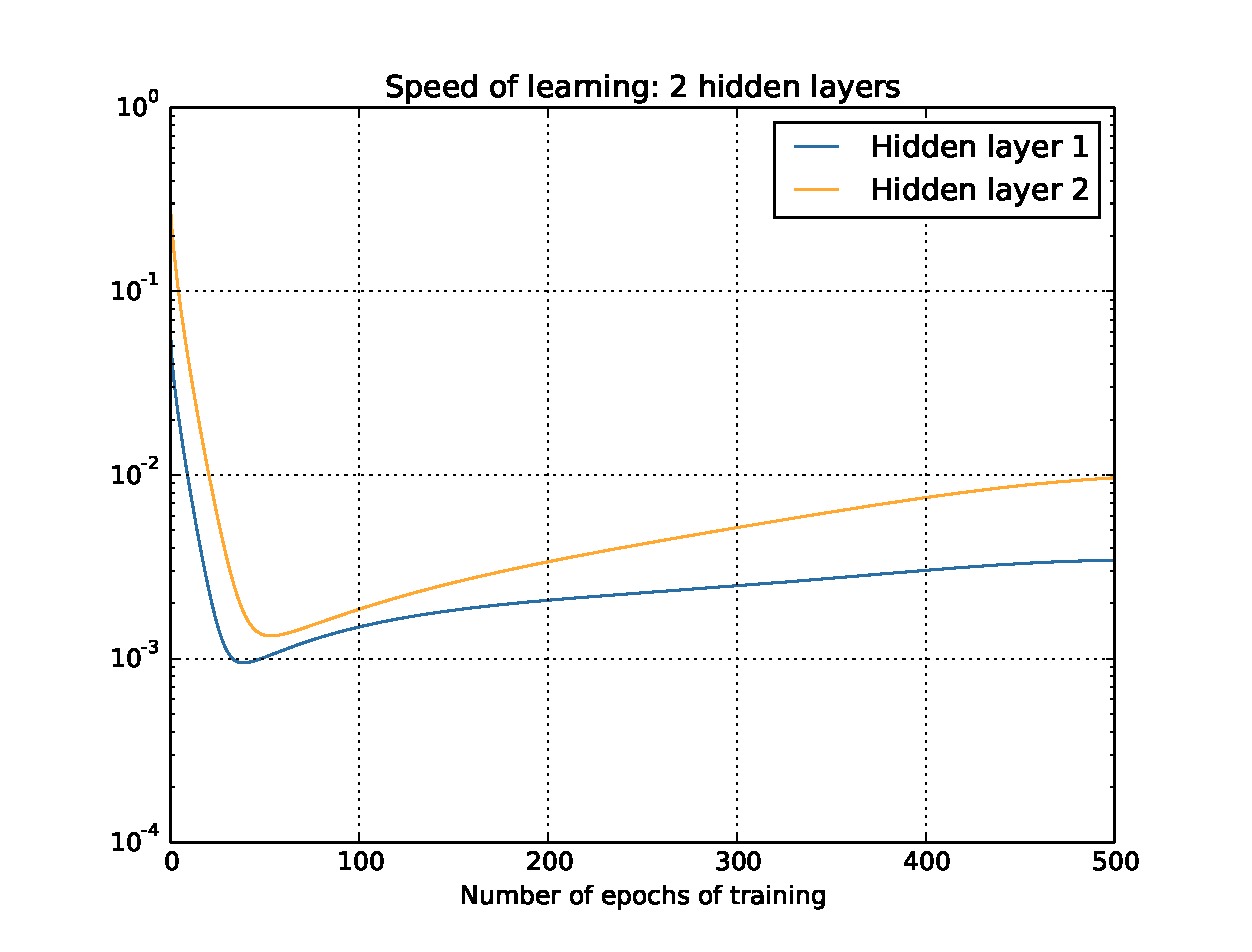
\includegraphics[width=.6\textwidth]{training_speed_2_layers}
\end{center}
 
为了产生这些结果,我在 $1000$ 个训练图像上进行了 $500$ 轮 batch 梯度下降。这和我
们通常训练方式还是不同的~——~我没有使用 minibatch,仅仅使用了 $1000$ 个训练图像,
而不是全部的 $50,000$ 幅图。我并不是想做点新鲜的尝试,或者蒙蔽你们的双眼,但因为
使用 minibatch 随机梯度下降会在结果中带来更多的噪声(尽管在平均噪声的时候结果很相
似)。使用我已经确定的参数可以对结果进行平滑,这样我们可以看清楚真正的情况是怎样
的。 如图所示,两层在开始时就有着不同的速度。然后两层的学习速度在触底前迅速下落。
在最后,我们发现第一层的学习速度变得比第二层更慢了。
 
那么更加复杂的网络是什么情况呢?这里是一个类似的实验,但是这次有三个隐藏层
($[784, 30, 30, 30, 10]$):
\begin{center}
  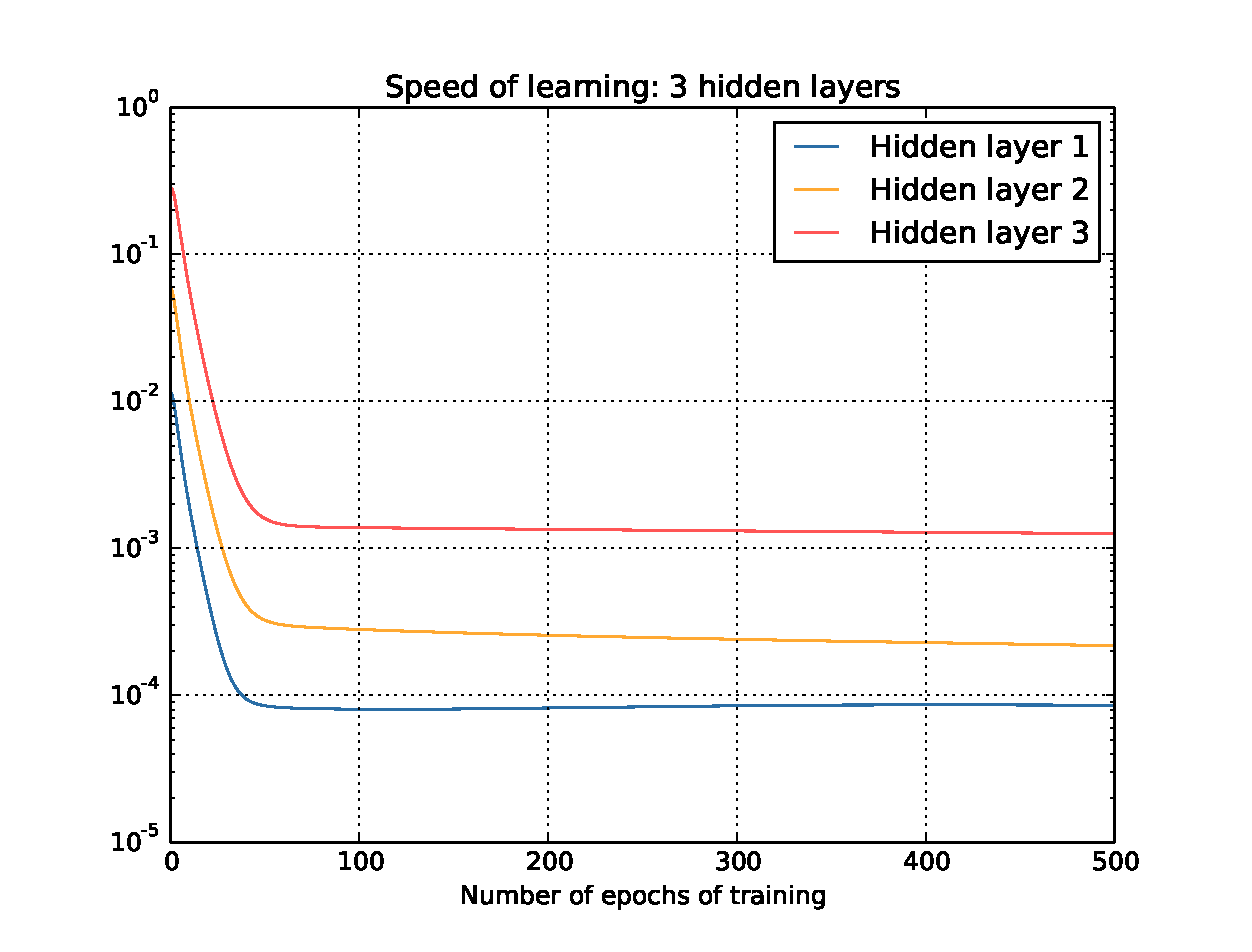
\includegraphics[width=.6\textwidth]{training_speed_3_layers}
\end{center}
 
同样,前面的隐藏层要比后面的隐藏层学习的更慢。最后一个实验,就是增加第四个隐藏层
($[784, 30, 30, 30, 30, 10]$),看看这里会发生什么:
\begin{center}
  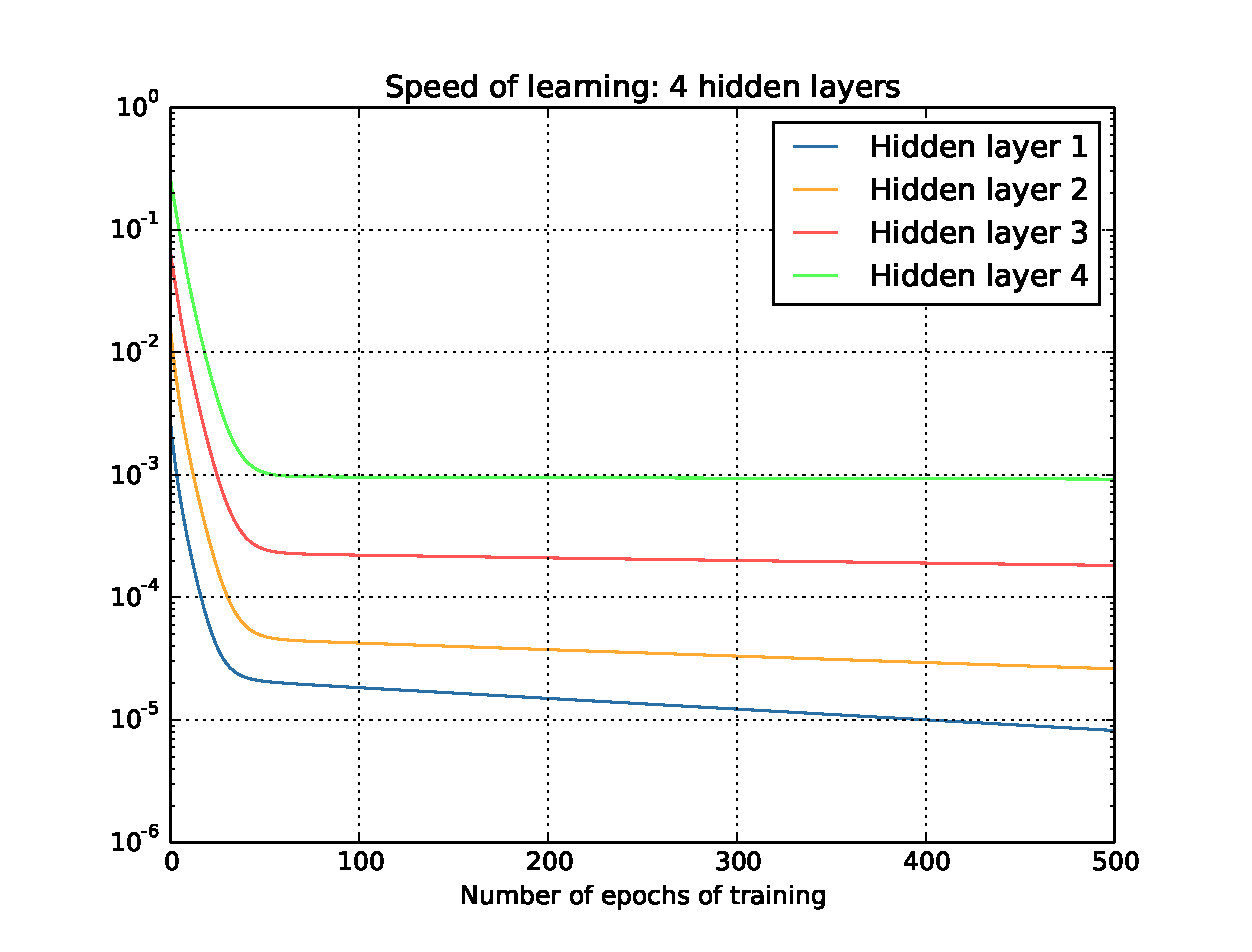
\includegraphics[width=.6\textwidth]{training_speed_4_layers}
\end{center}
 
同样的情况出现了,前面的隐藏层的学习速度要低于后面的隐藏层。这里,第一层的学习速
度和最后一层要差了两个数量级,也就是比第四层慢了 $100$ 倍。难怪我们之前在训练这些
网络的时候遇到了大麻烦!
 
现在我们已经有了一项重要的观察结果:至少在某些深度神经网络中,在我们在隐藏层 BP的
时候梯度倾向于变小。这意味着在前面的隐藏层中的神经元学习速度要慢于后面的隐藏层。
这儿我们只在一个网络中发现了这个现象,其实在多数的神经网络中存在着更加根本的导致
这个现象出现的原因。这个现象也被称作是\emph{消失的梯度问题\index{消失的梯度问
    题}(vanishing gradient
  problem)}\footnote{参见
  \href{http://citeseerx.ist.psu.edu/viewdoc/summary?doi=10.1.1.24.7321}{Gradient
    flow in recurrent nets: the difficulty of learning long-term dependencies},
  作者为 Sepp Hochreiter,Yoshua Bengio, Paolo Frasconi, 和 Jürgen
  Schmidhuber (2001)。这篇论文研究了递归神经网络,但是其本质现象和我们正在研究
  的前馈网络中的是一样的。还可看看 Sepp Hochreiter的早期的学位论
  文,
  \href{http://www.idsia.ch/~juergen/SeppHochreiter1991ThesisAdvisorSchmidhuber.pdf}{Untersuchungen
    zu dynamischen neuronalen Netzen} (1991,德语)。}。
 
为何消失的梯度问题会出现呢?我们可以通过什么方式避免它?还有在训练深度神经网络时
如何处理好这个问题?实际上,这个问题是可以避免的,尽管替代方法并不是那么有效,同
样会产生问题~——~在前面的层中的梯度会变得非常大!这也叫做\emph{激增的梯度问
  题}(\emph{exploding gradient problem}),这也没比消失的梯度问题更好处理。更加
一般地说,在深度神经网络中的梯度是\emph{不稳定}的,在前面的层中或会消失,或会激增。
这种不稳定性才是深度神经网络中基于梯度学习的根本问题。这就是我们需要理解的东西,
如果可能的话,采取合理的步骤措施解决问题。
 
一种有关消失的(不稳定的)梯度的看法是确定这是否确实是一个问题。此刻我们暂时转换
到另一个话题,假设我们正要数值优化一个一元的函数 $f(x)$。如果其导数 $f'(x)$ 很小,
这难道不是一个好消息么?是不是意味着我们已经接近极值点了?同样的方式,在深度神经
网络中前面隐藏层的小的梯度是不是表示我们不需要对权重和偏置做太多调整了?
 
当然,实际情况并不是这样的。想想我们随机初始网络中的权重和偏置。在面对任意的一种
任务,单单使用随机初始的值就能够获得一个较好的结果是太天真了。具体讲,看
看 MNIST问题的网络中第一层的权重。随机初始化意味着第一层丢失了输入图像的几乎所有
信息。即使后面的层能够获得充分的训练,这些层也会因为没有充分的信息而很难识别出输
入的图像。因此,在第一层不进行学习的尝试是不可能的。如果我们接着去训练深度神经网
络,我们需要弄清楚如何解决消失的梯度问题。

\section{什么导致了消失的梯度问题?深度神经网络中的梯度不稳定性}
\label{sec:what_is_causing_the_vanishing_gradient_problem_unstable_gradients_in_deep_neural_nets}

为了弄清楚为何会出现消失的梯度,来看看一个极简单的深度神经网络:每一层都只有一个
单一的神经元。下图就是有三层隐藏层的神经网络:
\begin{center}
  \includegraphics{tikz37}
\end{center}

这里,$w_1, w_2, \ldots$ 是权重,而 $b_1, b_2, \ldots$ 是偏置,$C$ 则是某个代价函
数。回顾一下,从第 $j$ 个神经元的输出 $a_j = \sigma(z_j)$,其中 $\sigma$ 是通常
的 \hyperref[sigmoid_neurons]{S 型激活函数},而 $z_j = w_j * a_{j-1} + b_j$ 是神
经元的带权输入。我已经在最后表示出了代价函数 $C$ 来强调代价是网络输出 $a_4$ 的函
数:如果实际输出越接近目标输出,那么代价会变低;相反则会变高。
 
现在我们要来研究一下关联于第一个隐藏神经元梯度 $\partial C/\partial b_1$。我们将
会计算出 $\partial C/\partial b_1$ 的表达式,通过研究表达式来理解消失的梯度发生的
原因。
 
开始就简单地给出 $\partial C/\partial b_1$ 的表达式。初看起来有点复杂,但是其结构
是相当简单的,我一会儿会解释。下图给出了具体的表达式:
\begin{center}
  \includegraphics{tikz38}
\end{center}

表达式结构如下:对每个神经元有一个 $\sigma'(z_j)$ 项;对每个权重有一个 $w_j$ 项;
还有一个 $\partial C/\partial a_4$ 项,表示最后的代价函数。注意,我已经将表达式中
的每个项置于了对应的位置。所以网络本身就是表达式的解读。
 
你可以直接认可这个表达式,直接跳到该表达式如何关联于小时的梯度问题的。这对理解没
有影响,因为实际上上面的表达式只是前面对于反向传播的讨论的特例。但是也包含了一个
表达式正确的解释,所以去看看那个解释也是很有趣的(也可能更有启发性吧)。
 
假设我们对偏置 $b_1$ 进行了微小的调整 $\Delta b_1$。这会导致网络中剩下的元素一系
列的变化。首先会对第一个隐藏元输出产生一个 $\Delta a_1$ 的变化。这样就会导致第二
个神经元的带权输入产生 $\Delta z_2$ 的变化。从第二个神经元输出随之发生 $\Delta
a_2$ 的变化。以此类推,最终会对代价函数产生 $\Delta C$ 的变化。这里我们有:
\begin{equation}
  \frac{\partial C}{\partial b_1} \approx \frac{\Delta C}{\Delta b_1}
  \label{eq:114}\tag{114}
\end{equation}

这表示我们可以通过仔细追踪每一步的影响来搞清楚 $\partial C/\partial b_1$ 的表达式。 

现在我们看看 $\Delta b_1$ 如何影响第一个神经元的输出 $a_1$ 的。我们有 $a_1 =
\sigma(z_1) = \sigma(w_1 a_0 + b_1)$,所以有
\begin{align}
  \Delta a_1 & \approx 
  \frac{\partial \sigma(w_1 a_0+b_1)}{\partial b_1} \Delta b_1 \label{eq:115}\tag{115}\\
  & = \sigma'(z_1) \Delta b_1 \label{eq:116}\tag{116}
\end{align}
 
$\sigma'(z_1)$ 这项看起很熟悉:其实是我们上面关于 $\partial C/\partial b_1$
的表达式的第一项。直觉上看,这项将偏置的改变 $\Delta b_1$ 转化成了输出的变
化 $\Delta a_1$。$\Delta a_1$ 随之又影响了带权输入 $z_2 = w_2 * a_1 +
b_2$:
\begin{align}
  \Delta z_2 & \approx
  \frac{\partial z_2}{\partial a_1} \Delta a_1 \label{eq:117}\tag{117}\\
  & = w_2 \Delta a_1 \label{eq:118}\tag{118}
\end{align}

将 $\Delta z_2$ 和 $\Delta a_1$ 的表达式组合起来,我们可以看到偏置 $b_1$
中的改变如何通过网络传输影响到 $z_2$的:
\begin{equation}
  \Delta z_2 \approx \sigma'(z_1) w_2 \Delta b_1
  \label{eq:119}\tag{119}
\end{equation}
 
现在,又能看到类似的结果了:我们得到了在表达式 $\partial C/\partial b_1$ 的前
面两项。

以此类推下去,跟踪传播改变的路径就可以完成。在每个神经元,我们都会选择一
个 $\sigma'(z_j)$ 的项,然后在每个权重我们选择出一个 $w_j$ 项。最终的结果就
是代价函数中变化 $\Delta C$ 的相关于偏置 $\Delta b_1$ 的表达式:
\begin{equation}
  \Delta C \approx \sigma'(z_1) w_2 \sigma'(z_2) \ldots \sigma'(z_4)
  \frac{\partial C}{\partial a_4} \Delta b_1
\label{eq:120}\tag{120}
\end{equation}

除以 $\Delta b_1$,我们的确得到了梯度的表达式:
\begin{equation}
  \frac{\partial C}{\partial b_1} = \sigma'(z_1) w_2 \sigma'(z_2) \ldots
  \sigma'(z_4) \frac{\partial C}{\partial a_4}
\label{eq:121}\tag{121}
\end{equation}
 
\textbf{为何出现梯度消失:} 现在把梯度的整个表达式写下来:
\begin{equation}
  \frac{\partial C}{\partial b_1} = \sigma'(z_1) \, w_2 \sigma'(z_2) \, w_3
  \sigma'(z_3) \, w_4 \sigma'(z_4) \, \frac{\partial C}{\partial a_4}
  \label{eq:122}\tag{122}
\end{equation}
 
除了最后一项,该表达式是一系列形如 $w_j \sigma'(z_j)$ 的乘积。为了理解每个项的行
为,先看看下面的sigmoid 函数导数的图像:
\begin{center}
  \includegraphics{sigmoid_prime_graph}
\end{center}
 
该导数在 $\sigma'(0)=1/4$ 时达到最高。现在,如果我们使用标准方法来初始化网络中的
权重,那么会使用一个均值为 $0$ 标准差为 $1$ 的高斯分布。因此所有的权重通常会满足
$|w_j| < 1$。有了这些信息,我们发现会有 $w_j \sigma'(z_j) < 1/4$。并且在我们进行
了所有这些项的乘积时,最终结果肯定会指数级下降:项越多,乘积的下降的越快。**这里
我们敏锐地嗅到了消失的梯度问题的合理解释。
 
更明白一点,我们比较一下 $\partial C/\partial b_1$ 和一个更后面一些的偏置的梯度,
不妨设为 $\partial C/\partial b_3$。当然,我们还没有显式地给出这个表达式,但是计
算的方式是一样的。 
\begin{center}
  \includegraphics{tikz39}
\end{center}

两个表示式有很多相同的项。但是 $\partial C/\partial b_1$ 还多包含了两个项。由于
这些项都是 $< 1/4$ 的。所以 $\partial C/\partial b_1$ 会是 $\partial C/\partial
b_3$ 的 1/16 或者更小。这其实就是消失的梯度出现的本质原因了。

当然,这里并非严格的关于消失的梯度微调的证明而是一个不太正式的论断。还有一些可能
的产生原因了。特别地,我们想要知道权重 $w_j$ 在训练中是否会增长。如果会,项 $w_j
\sigma'(z_j)$ 会不会不在满足之前 $w_j \sigma'(z_j) < 1/4$ 的约束。事实上,如果项
变得很大——超过 1,那么我们将不再遇到消失的梯度问题。实际上,这时候梯度会在我们
BP 的时候发生指数级地增长。也就是说,我们遇到了梯度激增的问题。\\

\textbf{梯度激增问题:} 现在看看梯度激增如何出现的把。这里的例子可能不是那么自然:
固定网络中的参数,来确保产生激增的梯度。但是即使是不自然,也是包含了确定会产生爆
炸梯度(而非假设的可能)的特质的。
 
共两个步骤:首先,我们将网络的权重设置得很大,比如 $w_1 = w_2 = w_3 = w_4 = 100$。
然后,我们选择偏置使得 $\sigma'(z_j)$ 项不会太小。这是很容易实现的:方法就是选择
偏置来保证每个神经元的带权输入是 $z_j = 0$(这样 $sigma'(z_j) = 1/4$)。比如说,
我们希望 $z_1 = w_1 * a_0 + b_1$。我们只要把 $b_1 = -100 * a_0$ 即可。我们使用同
样的方法来获得其他的偏置。这样我们可以发现所有的项 $w_j * \sigma'(z_j)$ 都等于
$100*1/4 = 25$。最终,我们就获得了激增的梯度。\\
 
\textbf{不稳定的梯度问题:} 根本的问题其实并非是消失的梯度问题或者激增的梯度问题,
而是在前面的层上的梯度是来自后面的层上项的乘积。当存在过多的层次时,就出现了内在
本质上的不稳定场景。唯一让所有层都接近相同的学习速度的方式是所有这些项的乘积都能
得到一种平衡。如果没有某种机制或者更加本质的保证来达成平衡,那网络就很容易不稳定
了。简而言之,真实的问题就是神经网络受限于\emph{不稳定梯度的问题}。所以,如果我们
使用标准的基于梯度的学习算法,在网络中的不同层会出现按照不同学习速度学习的情况。

\subsection*{练习}

\begin{itemize}
\item 在我们对于消失的梯度问题讨论中,使用了 $|\sigma'(z)| < 1/4$ 这个结论。假设
  我们使用一个不同的激活函数,其导数值是非常大的。这会帮助我们避免不稳定梯度的问
  题么?
\end{itemize}
 
\textbf{消失的梯度问题普遍存在:} 我们已经看到了在神经网络的前面的层中梯度可能会
消失也可能会爆炸。实际上,在使用 sigmoid 神经元时,梯度通常会消失。为什么?再看看
表达式 $|w\sigma'(z)|$。为了避免消失的梯度问题,我们需要 $|w\sigma'(z)| >= 1$。你
可能会认为如果 $w$ 很大的时候很容易达成。但是这比看起来还是困难很多。原因在
于,$\sigma'(z)$ 项同样依赖于 $w$:$\sigma'(z) = \sigma'(w*a+b)$,其中 $a$ 是输入
的激活函数。所以我们在让 $w$ 变大时,需要同时不让 $\sigma'(wa+b)$ 变小。这将是很
大的限制了。原因在于我们让 $w$ 变大,也会使得 $wa + b$ 变得非常大。看
看 $\sigma'$ 的图,这会让我们走到 $\sigma'$ 的两翼,这里会去到很小的值。唯一避免
发生这个情况的方式是,如果输入激活函数掉入相当狭窄的范围内(这个量化的解释在下面
第一个问题中进行)。有时候,有可能会出现。但是一般不大会发生。所以一般情况下,会
遇到消失的梯度。

\subsection*{问题}

\begin{itemize}
\item 考虑乘积 $|w\sigma'(wa+b)|$。假设有 $|w\sigma'(wa+b)| >= 1$。(1)这种情况
  只有在 $|w| >= 4$ 的时候才会出现。(2)假设 $|w| >= 4$,考虑那些满
  足 $|w\sigma'(wa+b)| >= 1$ 的输入激活 $a$ 集合。证明:满足上述条件的该集合能够
  充满一个不超过 $\frac{2}{|w|}\ln(\frac{|w|(1+\sqrt{1-4/|w|})}{2}-1)$ 宽度的区间。
  (3)数值上说明上述表达式在 $|w| ~= 6.9$ 时候去的最高值约
  $0.45$。所以即使每个条件都满足,我们仍然有一个狭窄的输入激活区间,这样来避免消
  失的梯度问题。
\item \textbf{幺神经元:}\label{identity_neuron} 考虑一个单一输入的神经元,$x$,
  对应的权重 $w_1$,偏差 $b$,输出上的权重 $w_2$。证明,通过合理选择权重和偏差,
  我们可以确保 $w_2 \sigma(w_1*x +b)~=x$
  其中$x \in [0, 1]$。这样的神经元可用来作为幺元使用,输出和输入相同(成比例
  )。\emph{提示:可以重写 $x = 1/2 + \Delta$,可以假设 $w_1$ 很小,和在 $w_1 *
    \Delta$ 使用泰勒级数展开}。
\end{itemize}

\section{在更加复杂网络中的不稳定梯度}

现在已经研究了简单的网络,每一层只包含一个神经元。那么那些每层包含很多神经元的更
加复杂的深度网络呢?
\begin{center}
  \includegraphics{tikz40}
\end{center}
 
实际上,在这样的神经网络中,同样的情况也会发生。在前面关于反向传播的章节中,我们
看到了在一个共 $L$ 层的第 $l$ 层的梯度:
\begin{equation}
  \delta^l = \Sigma'(z^l) (w^{l+1})^T \Sigma'(z^{l+1}) (w^{l+2})^T \ldots
  \Sigma'(z^L) \nabla_a C
  \label{eq:124}\tag{124}
\end{equation}

这里 $\Sigma'(z^l)$ 是一个对角矩阵,每个元素是对第 $l$ 层的带权输入 $\sigma'(z)$。
而 $w^l$ 是对不同层的权值矩阵。$\nabla_{a} C$ 是对每个输出激活的偏导数向量。
 
这是更加复杂的表达式。不过,你仔细看,本质上的形式还是很相似的。主要是包含了更多
的形如 $(w^j)^T \Sigma' (z^j)$ 的对 (pair)。而且,矩阵 $\Sigma'(z^j)$ 在对角线上
的值挺小,不会超过 $1/4$。由于权值矩阵 $w^j$ 不是太大,每个额外的项 $(w^j)^T
\sigma' (z^l)$ 会让梯度向量更小,导致梯度消失。更加一般地看,在乘积中大量的项会导
致不稳定的梯度,和前面的例子一样。实践中,一般会发现在 sigmoid网络中前面的层的梯
度指数级地消失。所以在这些层上的学习速度就会变得很慢了。这种减速不是偶然现象:也
是我们采用的训练的方法决定的。

\section{其它深度学习的障碍}

本章我们已经聚焦在消失的梯度上,并且更加一般地,不稳定梯度~——~深度学习的一大障碍。
实际上,不稳定梯度仅仅是深度学习的众多障碍之一,尽管这一点是相当根本的。当前的研
究集中在更好地理解在训练深度神经网络时遇到的挑战。这里我不会给出一个详尽的总结,
仅仅想要给出一些论文,告诉你人们正在寻觅探究的问题。
 
首先,
在 2010 年 Glorot 和
Bengio\footnote{\href{http://jmlr.org/proceedings/papers/v9/glorot10a/glorot10a.pdf}{Understanding
    the difficulty of training deep feedforward neural networks},作者为 Xavier
  Glorot 和 Yoshua Bengio(2010)。还可看
  看 \href{http://yann.lecun.com/exdb/publis/pdf/lecun-98b.pdf}{Efficient
    BackProp} 论文中前面的关于 S 型函数的讨论,作者为 Yann LeCun, Léon
  Bottou, Genevieve Orr 和 Klaus-Robert Müller(1998)。} 发现证据表明 sigmoid
函数的选择会导致训练网络的问题。特别地,他们发现 sigmoid 函数会导致最终层上的激活
函数在训练中会聚集在 $0$,这也导致了学习的缓慢。他们的工作中提出了一些取
代 sigmoid 函数的激活函数选择,使得不会被这种聚集性影响性能。
 
第二个例子,在 2013 年 Sutskever, Martens,
Dahl 和
Hinton\footnote{\href{http://www.cs.toronto.edu/~hinton/absps/momentum.pdf}{On
    the importance of initialization and momentum in deep learning},作者为 Ilya
  Sutskever,James Martens, George Dahl 和 Geoffrey Hinton (2013)。} 研究了深
度学习使用随机权重初始化和基于 momentum 的 $SGD$ 方法。两种情形下,好的选择可以获
得较大的差异的训练效果。

这些例子告诉我们,“什么让训练深度网络非常困难”这个问题相当复杂。本章,我们已经
集中于深度神经网络中基于梯度的学习方法的不稳定性。结果表明了激活函数的选择,权重
的初始化,甚至是学习算法的实现方式也扮演了重要的角色。当然,网络结构和其他超参数
本身也是很重要的。因此,太多因子影响了训练神经网络的难度,理解所有这些因子仍然是
当前研究的重点。尽管这看起来有点悲观,但是在下一章中我们会介绍一些好的消息,给出
一些方法来一定程度上解决和迂回所有这些困难。
